% ---
% id: kempe-chains
% title: Kempe 사슬 이용
% status: in-progress
% parent: five-color
% alternatives: [discharging]
% concepts: [euler-formula, kempe-chain]
% next: 꼭짓점 순서를 바꿔도 식 (1)이 유지되는지 확인
% created: 2026-09-30
% topics: [coloring]
% kind: calc
% description: "꼭짓점 순서를 바꿔도 식 (1)이 유지되는지 계산으로 확인"
% ---
\section{5색 정리: Kempe 사슬을 이용한 접근}
% 근거: docs/note/chapters/02-five-color.tex

평면 그래프 $G-v$를 다섯 색으로 칠한 $c$에서 차수 5인 꼭짓점 $v$의 이웃 $v_1,\dots,v_5$가 다섯 색을 모두 쓰고
\begin{equation}\label{eq:kempe}
  v_3 \notin \kc{1}{3}{v_1}, \quad c(v_1) \ne c(v_3)
\end{equation}
이면, 다음을 만족하는 다시 칠한 색칠 $c'$이 존재한다.
\begin{equation}\label{eq:recolor}
  c'(v_1) = c(v_3), \quad c'(v_3) = c(v_3).
\end{equation}

% 확인할 것: 꼭짓점 순서를 바꿔도 \eqref{eq:kempe}가 유지되는가
\begin{figure}[h]
  \centering
  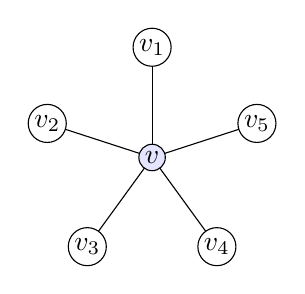
\begin{tikzpicture}
    \foreach \i in {1,...,5} \draw (0,0) -- ({90+72*(\i-1)}:1.4) node[circle,draw,fill=white,inner sep=1pt] {$v_\i$};
    \node[circle,draw,fill=blue!10,inner sep=1pt] at (0,0) {$v$};
  \end{tikzpicture}
  \caption{차수 5인 꼭짓점 $v$와 이웃 다섯 $v_1,\dots,v_5$.}
\end{figure}

식 \eqref{eq:recolor}의 $c'$으로 네 색만 쓸 수 있는지는 아직 확인하지 않았다.
